% Row 5 (training dynamics + takeaways + QR/paper link), removed from the poster for space.
% To restore: paste this back into blade-poster.tex above the "Row 6: references" marker.
      % ======================= Row 5: dynamics + takeaways =======================
      \begin{columns}[T]
        \begin{column}{0.62\linewidth}
          \begin{psublock}[equal height group=r5]{{Smooth, self-correcting training dynamics}}
            \begin{columns}[T]
              \begin{column}{0.49\linewidth}
                \centering\textbf{\method:} three phases\\[0.3ex]
                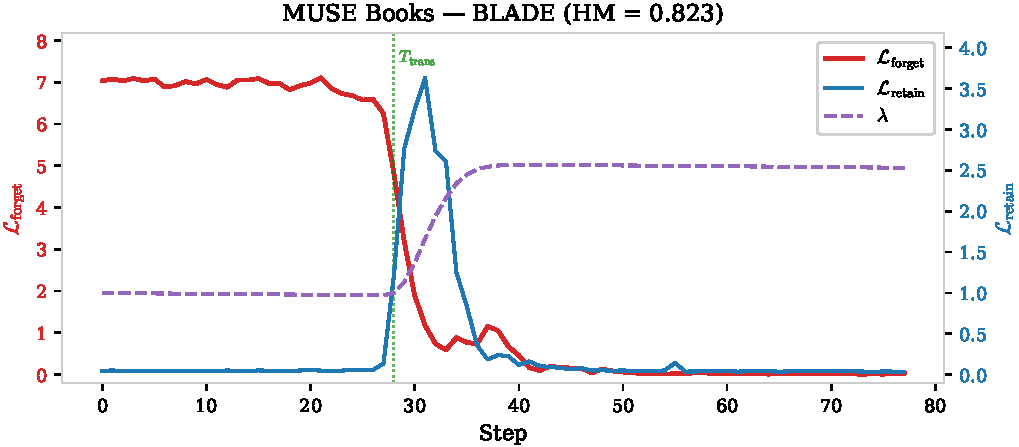
\includegraphics[width=\linewidth]{figures/fig_muse_books_dynamics}
              \end{column}
              \begin{column}{0.49\linewidth}
                \centering\textbf{PDU:} recurring oscillations\\[0.3ex]
                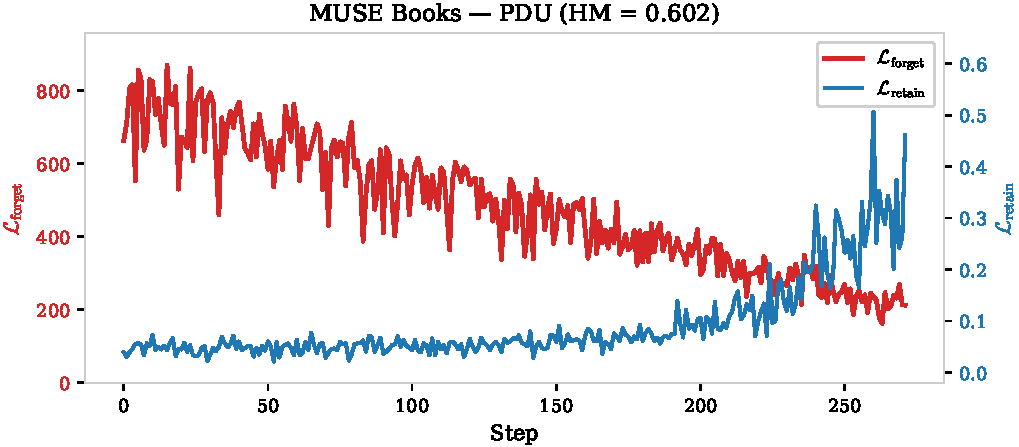
\includegraphics[width=\linewidth]{figures/fig_muse_books_PDU_dynamics}
              \end{column}
            \end{columns}
            \vspace{1ex}
            \centering% BLADE's three training phases (paper, Training Dynamics).
\begin{tikzpicture}[
    phase/.style={draw=psu-beaver, fill=psu-beaver-tint, line width=2.5pt, rounded corners=10pt,
      minimum height=1.7cm, align=center, inner xsep=14pt, font=\bfseries},
    flow/.style={-{Triangle[length=14pt,width=16pt]}, line width=3.5pt, color=psu-beaver},
  ]
  \node[phase] (a) {Warm-up};
  \node[phase, right=1.6cm of a] (b) {Spike \& ratchet: $\lambda$ up for good};
  \node[phase, right=1.6cm of b] (c) {Smooth convergence};
  \draw[flow] (a) -- (b);
  \draw[flow] (b) -- (c);
\end{tikzpicture}

          \end{psublock}
        \end{column}
        \begin{column}{0.36\linewidth}
          \begin{psufinalblock}{Takeaways and limitations}
            \setlength{\tabcolsep}{4pt}\renewcommand{\arraystretch}{1.3}
            \begin{tabular}{@{}c@{\ \ }p{0.88\linewidth}@{}}
              {\color{psu-beaver}\faCheck} & \circnum{3} \textbf{Bounded}, self-decelerating forget loss \\
              {\color{psu-beaver}\faCheck} & \circnum{1}\,\circnum{2} \textbf{Adaptive} retain protection \\
              {\color{psu-beaver}\faCheck} & \textbf{LoRA} bounds representational drift \\
              {\color{psu-beaver}\faCheck} & \textbf{Stable:} $4\times$ scale, 4 sequential requests \\
              {\color{psu-pink}\faIcon{exclamation-triangle}} & \textbf{Limitation:} re-learning attacks \\
              {\color{psu-pink}\faIcon{exclamation-triangle}} & \textbf{Not yet tested:} concept-level, multimodal \\
            \end{tabular}
          \end{psufinalblock}

          \begin{plainblock}{}
            \begin{columns}[c]
              \begin{column}{0.16\linewidth}
                \qrcode[height=\linewidth,hyperlink]{https://arxiv.org/pdf/2608.22557}
              \end{column}
              \begin{column}{0.82\linewidth}
                \raggedright
                {\large\bfseries\color{psu-beaver}Read the paper:} \href{https://arxiv.org/abs/2608.22557}{arXiv:2608.22557}\\[0.3ex]
                {\small To appear in \emph{EMNLP 2026}}\\
                {\small\textbf{Code:} \url{https://github.com/tzpranto/blade}}\\[0.5ex]
                {\tiny Supported in part by U.S. NSF awards \#2438810 and \#2555559, Amazon Nova AI challenge award, and PSU Frymoyer chairship award. Some experimental results were obtained using computational resources provided by CloudBank, supported through U.S. NAIRR award \#240336.\par}
              \end{column}
            \end{columns}
          \end{plainblock}
        \end{column}
      \end{columns}

